\documentclass[11pt,a4paper]{article}
\usepackage[T1]{fontenc}
\usepackage{lmodern}
\usepackage{amssymb,amsmath}
\usepackage{ifxetex,ifluatex}
\usepackage{fixltx2e} % provides \textsubscript
% use upquote if available, for straight quotes in verbatim environments
% \usepackage[sc,osf]{mathpazo}
\usepackage{helvet}
\renewcommand{\familydefault}{\sfdefault}
% \usepackage{crimson}
\IfFileExists{upquote.sty}{\usepackage{upquote}}{}
% \ifnum 0\ifxetex 1\fi\ifluatex 1\fi=0 % if pdftex
%   \usepackage[utf8]{inputenc}
% % \else % if luatex or xelatex
%   \ifxetex
%     \usepackage{mathspec}
%     \usepackage{xltxtra,xunicode}
%   \else
%     \usepackage{fontspec}
%   \fi
%   \defaultfontfeatures{Mapping=tex-text,Scale=MatchLowercase}
%   \newcommand{\euro}{€}
% % % % % \fi
% use microtype if available
\IfFileExists{microtype.sty}{\usepackage{microtype}}{}
% % % \usepackage{biblatex}
% 
\usepackage[backend=biber,style=authoryear-comp,natbib,sortcites=none,autopunct=true]{biblatex}
\renewcommand*{\nameyeardelim}{\addspace}


\usepackage{longtable,booktabs}



\usepackage{graphicx}
% Redefine \includegraphics so that, unless explicit options are
% given, the image width will not exceed the width of the page.
% Images get their normal width if they fit onto the page, but
% are scaled down if they would overflow the margins.
\makeatletter
\def\ScaleIfNeeded{%
  \ifdim\Gin@nat@width>\linewidth
    \linewidth
  \else
    \Gin@nat@width
  \fi
}
\makeatother
\let\Oldincludegraphics\includegraphics
{%
 \catcode`\@=11\relax%
 \gdef\includegraphics{\@ifnextchar[{\Oldincludegraphics}{\Oldincludegraphics[width=\ScaleIfNeeded]}}%
}%

% \ifxetex
%   \usepackage[setpagesize=false, % page size defined by xetex
%               unicode=false, % unicode breaks when used with xetex
%               xetex]{hyperref}
% \else
%   \usepackage[unicode=true]{hyperref}
% \fi

\usepackage[colorlinks=true, urlcolor=blue, linkcolor=black, citecolor=blue, pdfauthor={Adam La Caze}]{hyperref}



% \urlstyle{same}  % don't use monospace font for urls

\providecommand{\tightlist}{%
  \setlength{\itemsep}{0pt}\setlength{\parskip}{0pt}}

\setlength{\parindent}{0pt}
\setlength{\parskip}{6pt plus 2pt minus 1pt}
\linespread{1.05}

\setlength{\emergencystretch}{3em}  % prevent overfull lines
\setcounter{secnumdepth}{5}

\title{Pharmacist responsibilities when selling complementary medicines}
\author{}
\date{}
\def\UrlBreaks{\do\/\do-\do?}

\newcommand{\vers}{v0.1 \hfill \today}

\newcommand\T{\rule{0pt}{2.6ex}}       % Top strut
\newcommand\B{\rule[-1.2ex]{0pt}{0pt}} % Bottom struct

\addbibresource{library.bib} %only if using biblatex

\begin{document}
\maketitle

\begin{tabular}{ll} Adam La Caze & Lecturer\tabularnewline
& School of Pharmacy\tabularnewline
& The University of Queensland\tabularnewline
& a.lacaze@uq.edu.au\tabularnewline[10pt] Amber Salman Popattia & School of Pharmacy\tabularnewline
& The University of Queensland\tabularnewline
& amber.salmanpopattia@uqconnect.edu.au\tabularnewline[10pt] Laetitia Hattingh & Adjunct Associate Professor\tabularnewline
& School of Pharmacy and Pharmacology\tabularnewline
& Griffith University\tabularnewline
& L.Hattingh@griffith.edu.au\tabularnewline
\end{tabular}

\vfill
This is a draft report for the project \emph{Evaluating the
acceptability and feasibility of an ethical framework for the sale of
complementary medicines in community pharmacy} funded by an APSA
Research Grant 2019.

\bigskip
\textbf{Document}: \vers
\newpage 

\tableofcontents

\newpage

\section{Synopsis}\label{synopsis}

Many consumers choose to use complementary medicines and frequently
purchase their complementary medicines from community pharmacy.
Pharmacists tend to vary in their approach to the sale of complementary
medicines and recent media reports suggest that some pharmacies are
failing to meet community expectations regarding the advice they
provide. There is a need for clearer guidance for pharmacists regarding
their responsibilities when selling complementary medicines. The
investigators have developed an ethical framework for the sale of
complementary medicines in community pharmacy. This project evaluated
the acceptability and feasibility of implementing an ethical framework
for the sale of complementary medicines in community pharmacy developed
by the investigators. Seventeen community pharmacists participated in
four focus groups and six individual interviews. There was good
representation among participants in terms of gender, years of practice,
pharmacy location and script volume.

\section{Background}\label{background}

Complementary medicines are a \$4.9 billion dollar industry in
Australia, 41\% of which is sold through pharmacies
\autocite{ComplementaryMedicinesAustralia2018}. Consumers purchase
complementary medicines from pharmacies due to a trust in the quality of
the products and the availability of advice.{[}REF{]} However, recent
reports suggest that pharmacists are failing to meet community
expectations regarding the advice they provide on complementary
medicines \autocites{Bray2017}{Thompson2017}{Arnold2016}[.][]{King2017}
A contributing factor to this is that the responsibilities of
pharmacists when selling complementary medicines are not well
articulated. There is clear recognition that pharmacists should (i)
support consumer choice and (ii) provide advice that is informed by
evidence \autocites{InternationalPharmaceuticalFederation2014}{PSA2017}.
There is, however, very little guidance on what to do when these two
principles conflict. The conflict arises because many complementary
medicines lack rigorous evidence of effectiveness and yet can cause harm
through adverse effects, drug interactions and delayed treatment
\autocites{Myers2004}{Izzo2009}. In the absence of evidence of benefit,
evidence-based guidance suggests that pharmacists should avoid selling
complementary medicines \autocite{Ernst1996}. But removing complementary
medicines from community pharmacy removes the opportunity for
pharmacists to support consumers in the safe use of complementary
medicines. This project seeks to contribute to pharmacy practice by
developing clear and practical guidance to pharmacists regarding their
responsibilities when selling complementary medicines.

\textcite{SalmanPopattia2018} identify several gaps in the literature
examining the responsibilities of pharmacists selling complementary
medicines. The most striking of these is the lack of specific guidance
for pharmacists on the sale of complementary medicines. The expectations
of pharmacists and consumers regarding the sale of complementary
medicines are well described
\autocites{Iyer2016a}{Tran:2013kh}{Kanjanarach2011}. To the extent that
ethical considerations are discussed in this literature, the conflict
between supporting consumer choice, evidence-based practice and business
considerations are frequently identified but never resolved. Part of the
problem is the lack of an explicit ethical theory to guide
decision-making. The `four principles approach' of bioethical
principlism is implicit in many discussions, but the version that is
employed focuses on `ethics first-aid': the \emph{identification} of
ethical conflicts rather than resolution of the conflict
\autocites{Beauchamp2012}{Pullman2005}

The problems associated with the lack of specific guidance for
pharmacist responsibilities when selling complementary medicines is
highlighted by the current \emph{Code of ethics for pharmacists}
\autocite{PSA2017}. While the code provides the advice to support
consumer choice and to practice in accordance with evidence, it also
provides the directive that pharmacists will ``only purchase, supply or
promote any medicine, complementary medicine, herbal remedy or other
healthcare product where there is credible evidence of efficacy and the
benefit of use outweighs the risk''. This directive is in contrast with
current practice in which complementary medicines that lack credible
evidence of efficacy are frequently purchased and supplied. There is no
attempt to reconcile this disparity in the professional or academic
literature---no explicit argument for the directive provided in the
code, nor a counter-argument defending the routine sale of complementary
medicines that lack evidence of efficacy in community pharmacy.

Salmon Popattia and La Caze have developed an ethical framework that
provides specific guidance to pharmacists regarding their
responsibilities when selling complementary medicines (currently under
preparation for publication). Details of the framework are provided in
Appendix A, and an overview is provided below.

\section{A framework for pharmacist responsibilities when selling
complementary
medicines}\label{a-framework-for-pharmacist-responsibilities-when-selling-complementary-medicines}

There are three components to the framework: principle-based ethics
provides the theoretical foundations, a \emph{public health argument}
provides \emph{prima facie} support for the sale of complementary
medicines in community pharmacy, and specific responsibilities are
provided that ensure that pharmacists meet their obligations to the
public when selling complementary medicines.

\subsection{Principle-based ethics}\label{principle-based-ethics}

Principle-based ethics, and more specifically, the `four principles
approach' to bioethics advocated by \textcite{Beauchamp2012}, is
frequently employed in bioethics and professional ethics in health care.
The four principles are \emph{respect for autonomy},
\emph{beneficience}, \emph{non-maleficence}, and \emph{justice}. The
theory provides resources for further specifying these general
principles when they conflict in particular contexts. The
approach---using \emph{reflective equilibrium} and
\emph{specification}---provides a framework for responding to ethical
challenges by explicitly weighing up and resolving conflicts in general
principles based on salient details within the context {[}REF{]}.

The specific responsibilities provided by the framework were developed
by weighing up mid-level principles such as the need for pharmacists to
provide evidence-based care as well as to respect the health beliefs and
preferences of consumers. These mid-level principles can be derived from
more general guiding principles, such as ensuring positive health
outcomes in consumers (beneficence and non-maleficence) and respecting
autonomy. The framework seeks to resolve the conflicts that arise in
these principles in relation to pharmacists selling complementary
medicines.

\subsection{Public health argument}\label{public-health-argument}

The second component of the framework is a public health argument for
pharmacists selling complementary medicines. This argument is driven by
two key points. First, complementary medicines are regulated in
Australia (and most regions in the world) as being sufficiently safe for
self-care. Most complementary medicines available in community pharmacy
are \emph{listed} on the Australian Register of Therapeutic Goods
\autocite{TGA2019_listed}. This means that the complementary medicine
contains items that are on a list of low-risk ingredients, is
manufactured according to the principles of Good Manufacturing Practice,
and the only claims made regarding therapeutic use relate to the
maintenance and enhancement of health for non-serious, self-limiting
conditions. Listed medicines are available from a wide range of outlets,
including pharmacies, health food stores, and supermarkets. Many
consumers choose to use complementary medicines and are likely to
continue to do so even if they were not available in community
pharmacies.

Second, pharmacists are a highly accessible health professional with the
training and skills to provide guidance on the appropriate use of
complementary medicines. In particular, pharmacists have excellent
skills in being able to identify and resolve potential drug interactions
and to provide guidance regarding actual or potential adverse reactions.
Pharmacists tend to focus on this role in relation to complementary
medicines and consumers frequently identify this support as one of the
drivers for purchasing complementary medicines from community pharmacies
\autocites{Olatunde2010}{Kanjanarach2011}.

The combination of these points provides a \emph{prima facie} argument
in support of the sale of complementary medicines in community pharmacy.
However, for the argument to be compelling pharmacists and pharmacy
support staff need to be proactive regarding complementary medicines and
provide evidence-based advice to consumers. This is not always the case.
Some pharmacists are hesitant to discuss complementary medicines with
consumers, and some provide inaccurate or misleading information
regarding the likely benefits of complementary medicines
\autocites{SalmanPopattia2018}{Arnold2016}{Bray2017}. The specific
responsibilities of pharmacists when selling complementary medicines
outlined below seek to address these issues. The framework identifies
the responsibilities that pharmacists must meet in order to make a
positive contribution to health outcomes by selling complementary
medicines.

\subsection{Specific responsibilities}\label{specific-responsibilities}

The key responsibilities outlined by the framework are provided in
Table~\ref{responsibilities}. The responsibilities overlap in some
respects, but each articulates a specific responsibility for pharmacists
working in a community pharmacy and managing staff. The framework makes
a distinction between pharmacy staff making an \emph{explicit
recommendation} to take a complementary medicine, and selling
complementary medicines without an explicit recommendation. The
framework suggests that \emph{recommendations} for a complementary
medicine must be consistent with current best evidence, and all
\emph{sales} of a complementary medicine should be accompanied with an
\emph{offer} of advice from a pharmacist. If consumers take up that
offer of advice, a pharmacist must be available to provide that advice
and to provide sufficient information to the consumer such that they can
make an informed decision with regard to the purchase of the
complementary medicine. Since some consumers might refuse the offer of
advice from a pharmacy, it is the responsibility of the pharmacist to
have procedures in place to identify and act if a consumer is at
significant risk of harm from complementary medicines. Further advice
regarding the responsibilities outlined in the framework are available
in Appendix A.

\begin{table}
\centering
\begin{tabular}{p{0.8\linewidth}}
\hline\T
1. Pharmacists should provide evidence-based recommendations to the consumers regarding complementary medicines\\[10pt]
2. Pharmacists should train all staff in a pharmacy and ensure that they provide evidence-based recommendations regarding complementary medicines and seek advice of a pharmacist when required\\[10pt]
3. When providing advice, pharmacists should provide sufficient information for consumers to make informed decisions regarding complementary medicines\\[10pt]
4. Pharmacists should setup the pharmacy so that consumers are provided an offer of advice from a pharmacist and pharmacists should be available to provide that advice\\[10pt]
5. Pharmacists must be vigilant for possible harms related to complementary medicines and intervene if risk of harm is significant\B\\
\hline
\end{tabular}
\caption{The key responsibilities of pharmacists selling complementary medicines}
\label{responsibilities}
\end{table}


\section{Aim}\label{aim}

The \textbf{specific aim} of this project is to evaluate the
acceptability and feasibility of the proposed ethical framework for the
sale of complementary medicines in community pharmacy. The project also
sought to identify any barriers to the acceptance and/or implementation
of the framework in community pharmacy.

\section{Methods}\label{methods}

Australian community pharmacists were invited to participate in online
workshops via a videoconferencing platform in September and October
2019. Pharmacists were be recruited using social media, professional
organisations, and communication through the professional networks of
key community pharmacy banner groups. If necessary, purposive sampling
was to be employed to ensure that the age and gender distribution of
participants reflects the workforce and that participants are recruited
with different levels of experience and from different practice
environments (small independent pharmacies, large chains, and
discount-oriented pharmacies).

The workshops employed focus group methods to engage participants in
discussion regarding the sale of complementary medicines in community
pharmacies. Focus groups provide an opportunity to investigate complex
behaviours and motivations, to learn more about the degree of consensus
on a topic, and to gain feedback regarding new ideas
\autocites{Basch1987}{Knodel1993}. They are especially helpful to
understand group norms, meanings and processes \autocite{BarbourFG2011}.
Workshops were offered inside and outside of usual business hours using
video-conferencing software, Zoom. Conducting focus groups via
video-conference provided an opportunity to recruit participants from a
large geographical area. A number of strategies were employed to support
the success of conducting the focus group in an online environment,
these included seeking to arrange groups of 4--6 participants (limiting
larger groups), enabling video feeds and offering alternatives for those
with lower internet speeds \autocite{Gaiser2017}.

Participants received information about the framework prior to the
workshop and were asked to complete a short pre-workshop survey. The
objectives of the workshops were (i) to examine the range of views
community pharmacists have regarding their responsibilities when selling
complementary medicines; (ii) to assess perceived appropriateness and
feasibility of the developed ethical framework; (iii) to identify
organisational, professional and personal barriers to the acceptance
and/or implementation of the ethical framework, and (iv) to aid the
development of specific guidance for pharmacists in applying the ethical
framework. Discussion topics explored the context in which pharmacists
provide advice on complementary medicines within community pharmacy, and
the acceptability and feasibility of the proposed ethical framework. The
semi-structured interviews conducted with participants unable to join a
workshop followed the same structure.

All focus groups and interviews were conducted by AL who has experience
in qualitative research, facilitation of online groups and research and
teaching in ethical reasoning and decision-making in pharmacy practice.
It was made clear from the start of each focus group and interview that
the objective of the discussion was to understand the participants views
and how they varied. Participants were encouraged to share diverging
views and to debate topics in a respectful manner. The facilitator did
not share views during the focus groups or interviews. ASP was an
observer for most of the focus groups and interviews. AL and ASP
debriefed immediately following each focus group and interview and
prepared the summary that was sent to participants for comment.

The workshops and interviews were video and audio recorded. Focus groups
and interviews were transcribed verbatim. The transcripts were analysed
using the thematic analysis methods described by Braun and Clarke
\autocite*{Braun2016}. An inductive approach to coding was employed, and
themes were developed with a focus on addressing the research questions
in the study. Two investigators, AL and ASP, familiarized themselves
with the data and developed an initial coding scheme. This was refined
through discussion early in the analysis and then used to code the focus
groups and interviews. AL and ASP then identified and refine themes
individually first, and then as a group that included LH.

\section{Results}\label{results}

Seventeen community pharmacists participated in 4 workshops and 6
individual interviews. The workshops contained 2--4 participants and
went from 29 to 68 minutes in duration (median duration 42.5 minutes).
The duration of the interviews ranged from 17 to 34 minutes (median 21
minutes). Demographic features of the participants are provided in Table
2. Participants varied in terms of gender, years of practice and type of
pharmacy and typical script volume. More than a third of participants
worked in a regional or rural location.

\begin{table}[htb]
\centering
\begin{tabular}{llc}
\hline
\multicolumn{2}{l}{\textbf{Demographics}}                                                                                                                   & \textbf{N}  \T\B\\
\hline
Gender            & Male                                                                                                                           & 9  \T\\
                  & Female                                                                                                                         & 8  \\
Years of practice & 1--5                                                                                                                            & 5  \\
                  & 6--10                                                                                                                           & 6  \\
                  & 11--20                                                                                                                          & 3  \\
                  & 20+                                                                                                                            & 3  \\
Type of pharmacy  & Large shopping centre                                                                                                          & 5  \\
                  & Small local                                                                                                                    & 6  \\
                  & Extended hours                                                                                                                 & 3  \\
                  & Discount                                                                                                                       & 3  \\
Location          & Urban area                                                                                              & 11 \\
                  & Regional area  & 5  \\
                  & Rural area              & 1  \\
Script volume     & 0--50 prescriptions                                                                                                            & 1  \\
                  & 50--100 prescriptions                                                                                                          & 4  \\
                  & 100--200 prescriptions                                                                                                         & 1  \\
                  & 200--300 prescriptions                                                                                                         & 3  \\
                  & 300+ prescriptions                                                                                                             & 8\B\\
\hline
\end{tabular}
\caption{Demographic features of the participants}
\end{table}

The presurvey questions provide a snapshot of the participants views
about complementary medicines in terms of their day-to-day practice.
Most participants agreed with statements regarding providing advice to
consumers about complementary medicines as being part of their role, and
feeling positive about the advice they give to consumers regarding
complementary medicines. Participants were less likely to agree with
statements regarding their possession of the necessary knowledge and
skills in relation to complementary medicines, and a statement regarding
possessing the necessary time and resources to help consumers with
complementary medicines.

\begin{figure}
\centering
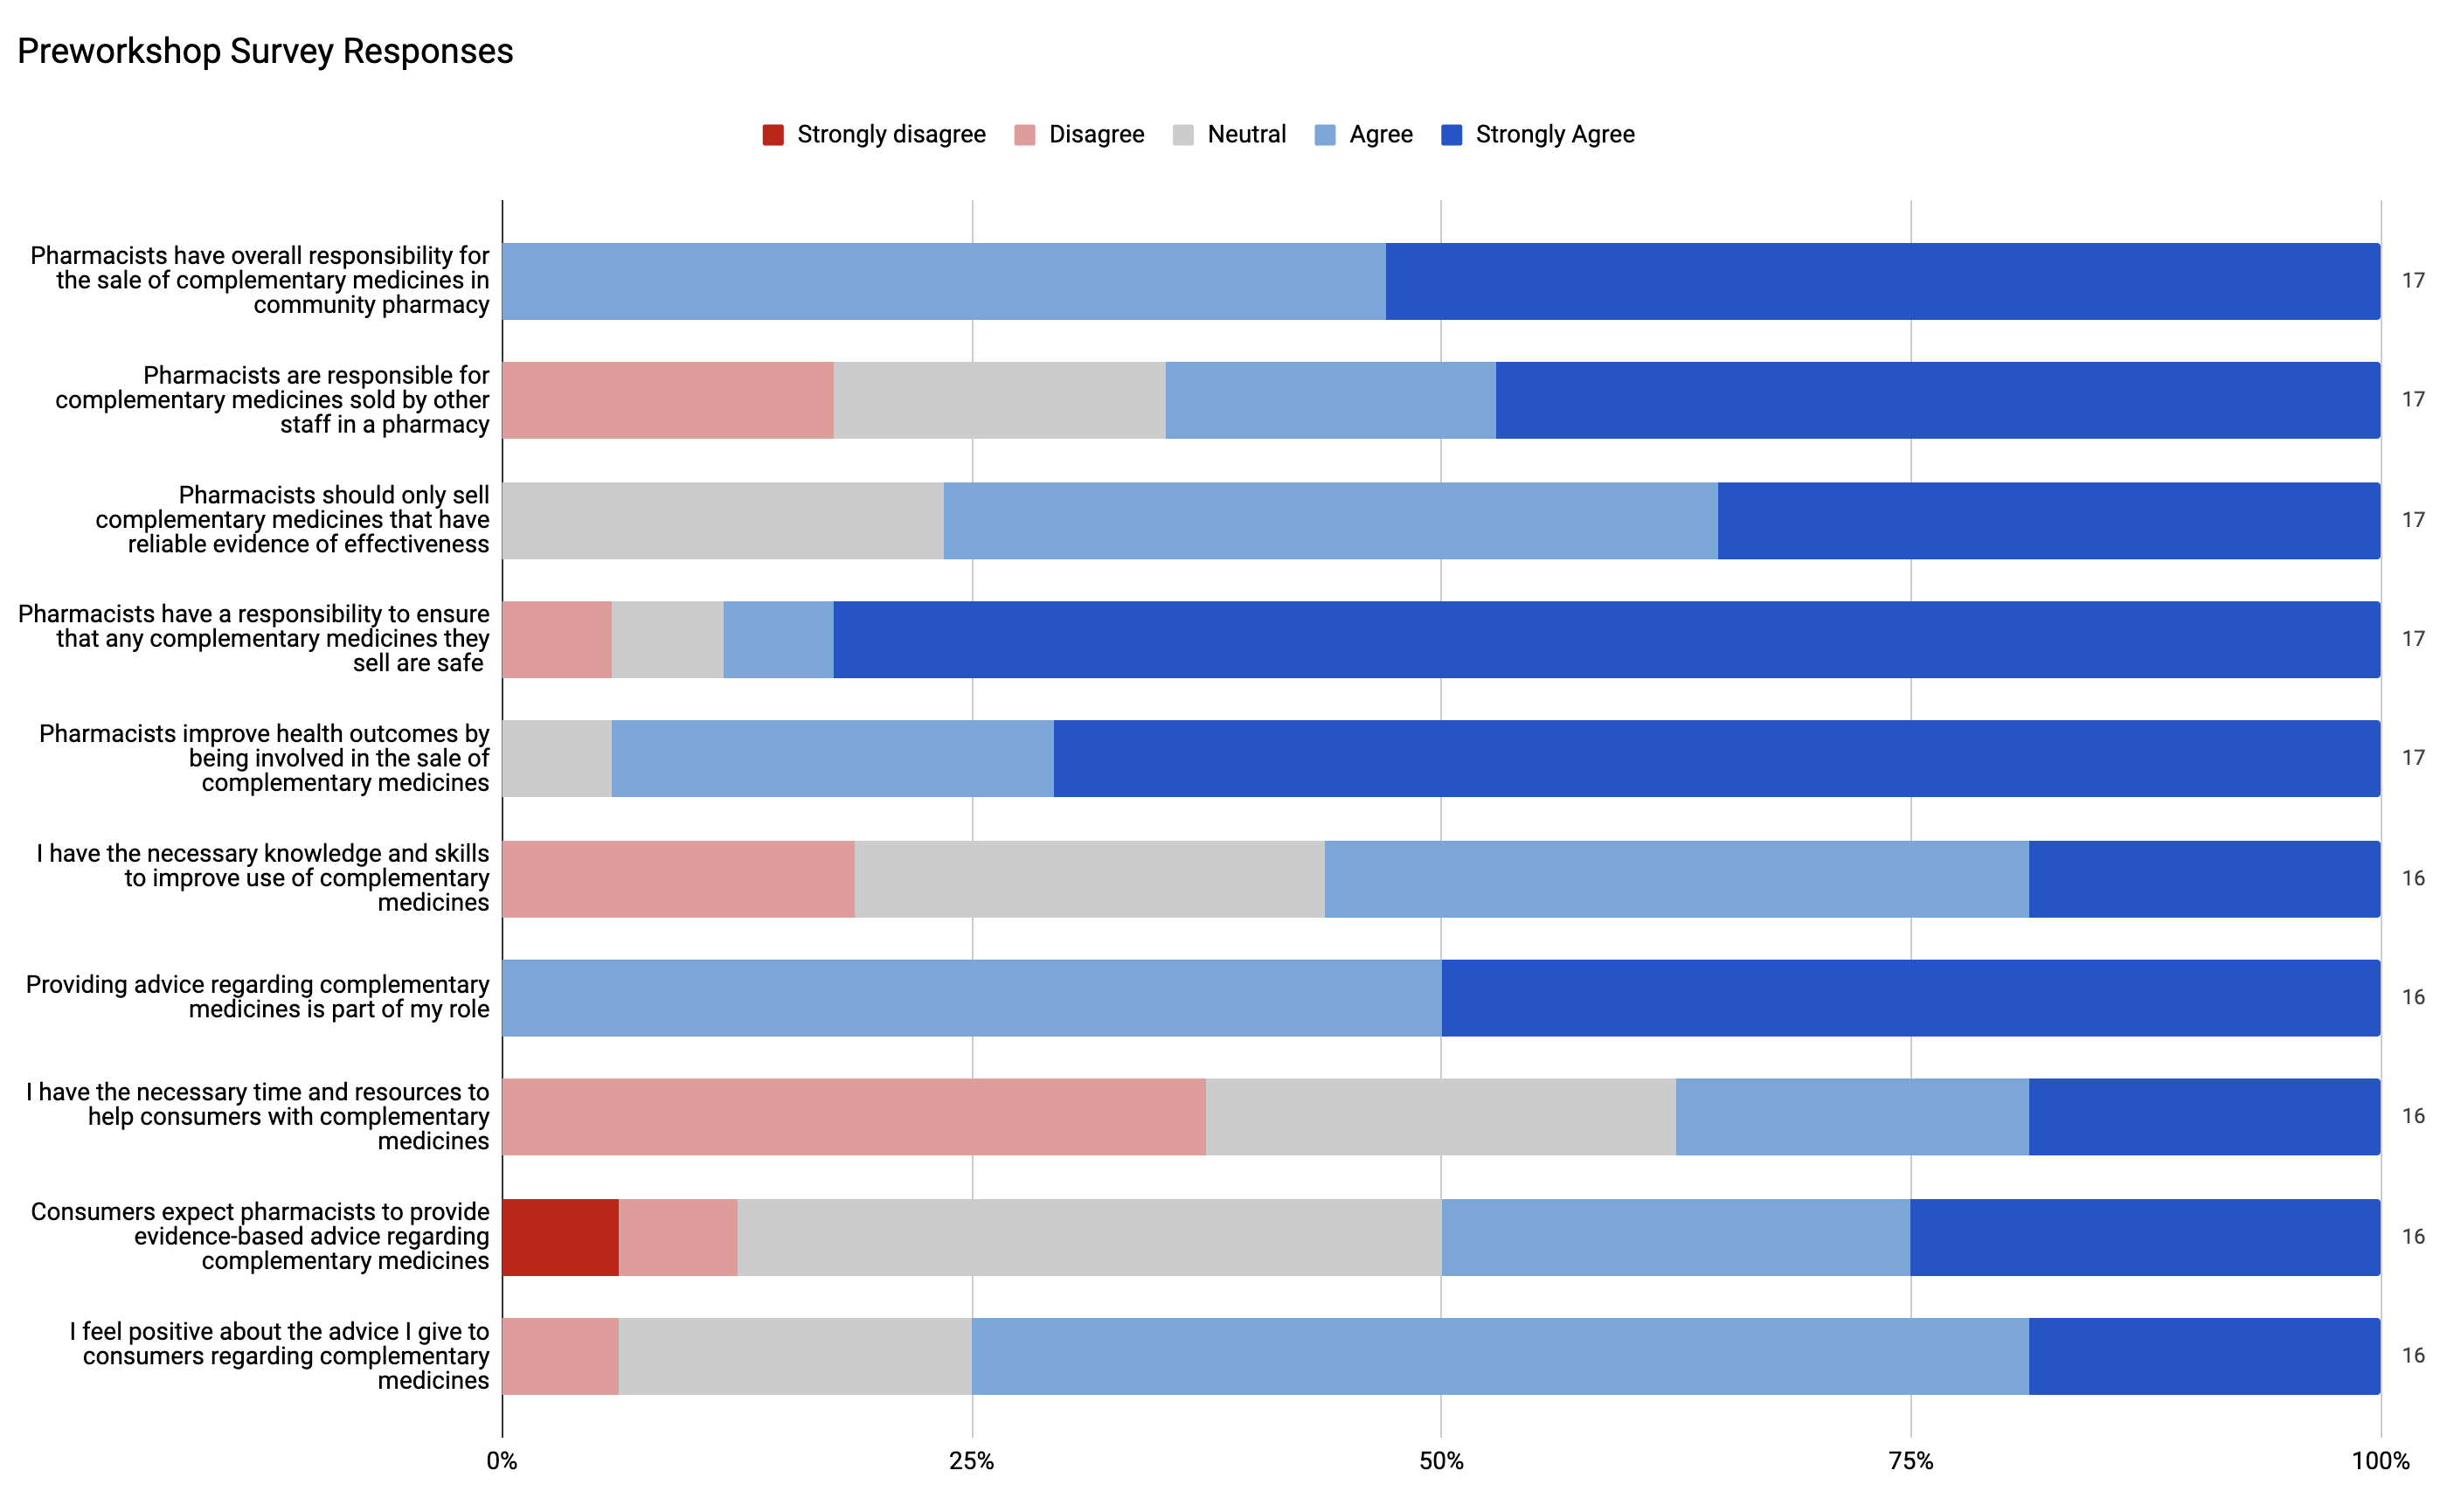
\includegraphics{fig_tab/presurvey.png}
\caption{Placeholder figure}
\end{figure}

\subsection{Key themes}\label{key-themes}

The focus groups provided rich information on how pharmacists approached
their practice in relation to complementary medicines, their perceptions
of the framework and the facilitators and barriers to implementing the
framework. Thematic saturation occurred after 3 focus groups and 4
interviews, additional focus groups and interviews helped to explore and
confirm key findings. Three main themes emerged from the focus groups
and interviews. These themes are summarised in Table 3. The first two
themes represent spectra on which participants differed: \emph{Approach
to complementary medicines (proactive--reactive)} and \emph{Approach to
evidence}. The third theme, \emph{Navigating practice in a retail
environment}, represents the recognition from all participants that
community pharmacy is in a retail environment and decisions regarding
professional practice have resource and other financial implications.

\begin{table}[tbh]
\centering
\begin{tabular}{>{\raggedright}p{0.5\linewidth}l}
\hline
\textbf{Theme}                               & \textbf{Relevance}\T\B\\
\hline
Approach to complementary medicines                 & Context, Feasibility       \T\\[21pt]
Approach to evidence  & Context, Acceptability     \\[10pt]
Navigating practice in a retail environment  & Acceptability, Feasibility\B\\
\hline
\end{tabular}
\caption{Key themes from the focus groups and interviews and the relevance these themes had on the context of complementary medicine sales in community pharmacy and the acceptability and feasibility of the proposed framework}
\end{table}

The ways in which participants \emph{approached complementary
medicines}, \emph{approached evidence}, and \emph{navigated practice in
a retail environment} inform how they viewed their responsibilities in
relation to complementary medicines within the context of community
pharmacy practice and their views on the acceptability and feasibility
of the proposed framework. Each of these themes are briefly introduced
below. Subsequent sections provide further discussion regarding how
participant responses within these themes addresses the objectives of
the project. Understanding these themes, and the ways in which
participants varied within the themes provide insight into the
\emph{context} (Section \ref{context}) of community pharmacy practice in
relation to complementary medicines, and the \emph{acceptability} and
\emph{feasibility} of the framework as perceived by the participants
(Section \ref{acceptability-and-feasibility-of-the-framework}).

\subsubsection{Approach to complementary
medicines}\label{approach-to-complementary-medicines}

A number of participants described their practice in terms of a
proactive approach to complementary medicines. These participants tended
to initiate discussion regarding complementary medicines with consumers
and see an important role for pharmacists in being active in relation to
complementary medicines.

\begin{quote}
Pharmacists are becoming more involved than before. People are trusting
pharmacists more. They always check their complementary medicine. I
think, from what I remember five years ago, people were just picking it
up. They were thinking that, ``That's just a supplement,'' but I think
the awareness is more than before among people. So they always come and
ask, ``Oh, is this one safe?'' or, ``What should I take?'' I think now,
lots of pharmacists are always checking things for them.
(D1P1)\footnote{Workshops and interviews are labelled as ``Discussions''
  and numbered in order. ``Participants'' are also allocated a number in
  order. ``D1P1'' refers to Discussion 1, Participant 1.}
\end{quote}

Some participants worked in community pharmacies set-up to provide
specialist advice on complementary medicines, including the use of
practitioner-lines.

\begin{quote}
I work in a small community pharmacy. I probably consider myself a
integrated pharmacist. We have complementary medicines in three
different areas similar to the rest of your medicines, like S2s, S3s. So
we've got some out in the front shop, which I consider your
{[}day-to-day{]} vitamins, like your supermarket lines. They're more
lines that are more for patients to choose and that sort of thing if
they want to self-select. If they go for advice from a pharmacist or
staff member, we'd probably go for something a bit better quality. So
we've got some in the S2 section which are, I guess, better quality
practitioner ranges. And then we've got your other ones in your S3 areas
which are ranges that do require a consult or a prescription. So a lot
of them are prescribed by some of our doctors as well. (D7P13)
\end{quote}

By contrast, other participants adopted a reactive approach to
complementary medicines. These participants indicated that they are less
likely to initiate discussion of complementary medicines with consumers,
and were more likely to express a lack of confidence in complementary
medicines. Participants expressing these views tended to rely more
heavily on support staff in this area.

\begin{quote}
I suppose it's not as big a focus in my professional practice\ldots{}. I
think it's probably because of lack of knowledge, to be honest, and
confidence, where you feel a lot more secure at the back counter or in a
dispensary than you do out in the vitamin section. (D5P8)
\end{quote}

For some participants, a reactive role towards complementary medicines
was seen as a consequence of the lack of evidence for the effectiveness
of many of these medicines.

\begin{quote}
Yeah. I think at the moment, I don't think we have much role to play in
selling or providing any counselling for complementary medicine because
first, working in community pharmacy, our main role is actually just
dispensing. And then pharmacies, I think, we should follow more like
evidence-based medicine practise\ldots{}. All this supplementary of
complementary medicine and all, they're not evidence-based. (D5P6)
\end{quote}

\subsubsection{Approach to evidence}\label{approach-to-evidence}

Participants also varied in their approach to evidence. Most, if not
all, participants explicitly endorsed ``evidence-based practice'' in
relation to complementary medicines, but what participants took this to
mean and how it related to their day-to-day practice tended to differ.

Many participants described their practice in a way that is consistent
with evidence-based practice while also recognising some of the
challenges.

\begin{quote}
{[}W{]}e shouldn't just be selling things because someone \ldots{} says,
``Oh, this turmeric is great for the sake of curing cancer.'' I think
there has to be some level of evidence\ldots{} And it's hard in certain
conditions because you're just never going to have the trials. (D4P5)
\end{quote}

A number of participants felt there should be a greater emphasis on
evidence-based practice in relation to complementary medicines.

\begin{quote}
If we, I think, perhaps as an industry, move towards more-- well, what
is the evidence? Do I feel that your needs will be met by what I'm
recommending today? Is there evidence to support what it says on the
label, or what it says in the marketing material? And if not, then maybe
we, as an industry, could push the emphasis of companies bringing things
to market, being more about actual evidence. More money going into these
studies of N equals 50. (D5P9)
\end{quote}

Some participants, however, expressed views inconsistent with
evidence-based practice. These participants put significantly more
weight into anecdotal reports and placebo effects as providing evidence
for the effectiveness of complementary medicines. In response to the
explicit PSA guidance to only sell complementary medicines that are
efficacious, one participant felt that placebo effects were sufficient
to meet this standard.

\begin{quote}
So how I would actually interpret {[}the PSA guidance{]}, and this is
where placebo effects comes in. So hey, if it's not doing them any harm
and they think it's better for them and they're going on in their life
and happy days, you just let them go. (D5P7)
\end{quote}

Other participants put a lot of value into anecdotal experience.

\begin{quote}
So I see a lot of people really---a lot of people want to use it. I've
talked to a lot of customers, and they do feel the result. Every time
they come back, I always ask, ``Is this working for you?'' And a lot of
times, they say, ``Yes, I know it's working because when my bottle ran
out, I started feeling it.'' So then they came back to get a new bottle.
So regarding your first question where you say, ``What's our perspective
regarding purchase of natural medications?'' I think they really work. I
think they work depending what the situation is. There are some
situations where you obviously need something more potent. But even in
those situations, I think there's always a place for natural medication,
either as a stand-alone treatment or in combination. This is just based
on what I've seen, not just what I think, what I've seen from what
people say. (D9P16)
\end{quote}

Participants tended to vary according to their approach to complementary
medicines and approach to evidence independently. Different participants
expressed each of the following views: ``proactive and evidence-based'',
``reactive and evidence-based'', ``proactive and less evidence-based''
and ``reactive and less evidence-based'' (see Figure~\ref{context3}).
Here, for example, is one of the participants suggesting that most
pharmacists they knew were ``reactive and evidence-based''

\begin{quote}
I would think in the most part people are very reactive. I don't know
that people would proactively engage in conversations a lot in my
experience. But I think if they were asked, then they would provide
evidence-based information to the best of their knowledge. (D6P10)
\end{quote}

Where participants exist on these spectra informed their response to a
variety of topics regarding the sale of complementary medicines in
community pharmacy, including the role of naturopaths, the availability
and confidence the participant had with regard to information resources,
practitioner-only products and the proposed framework.

\begin{figure}
\centering
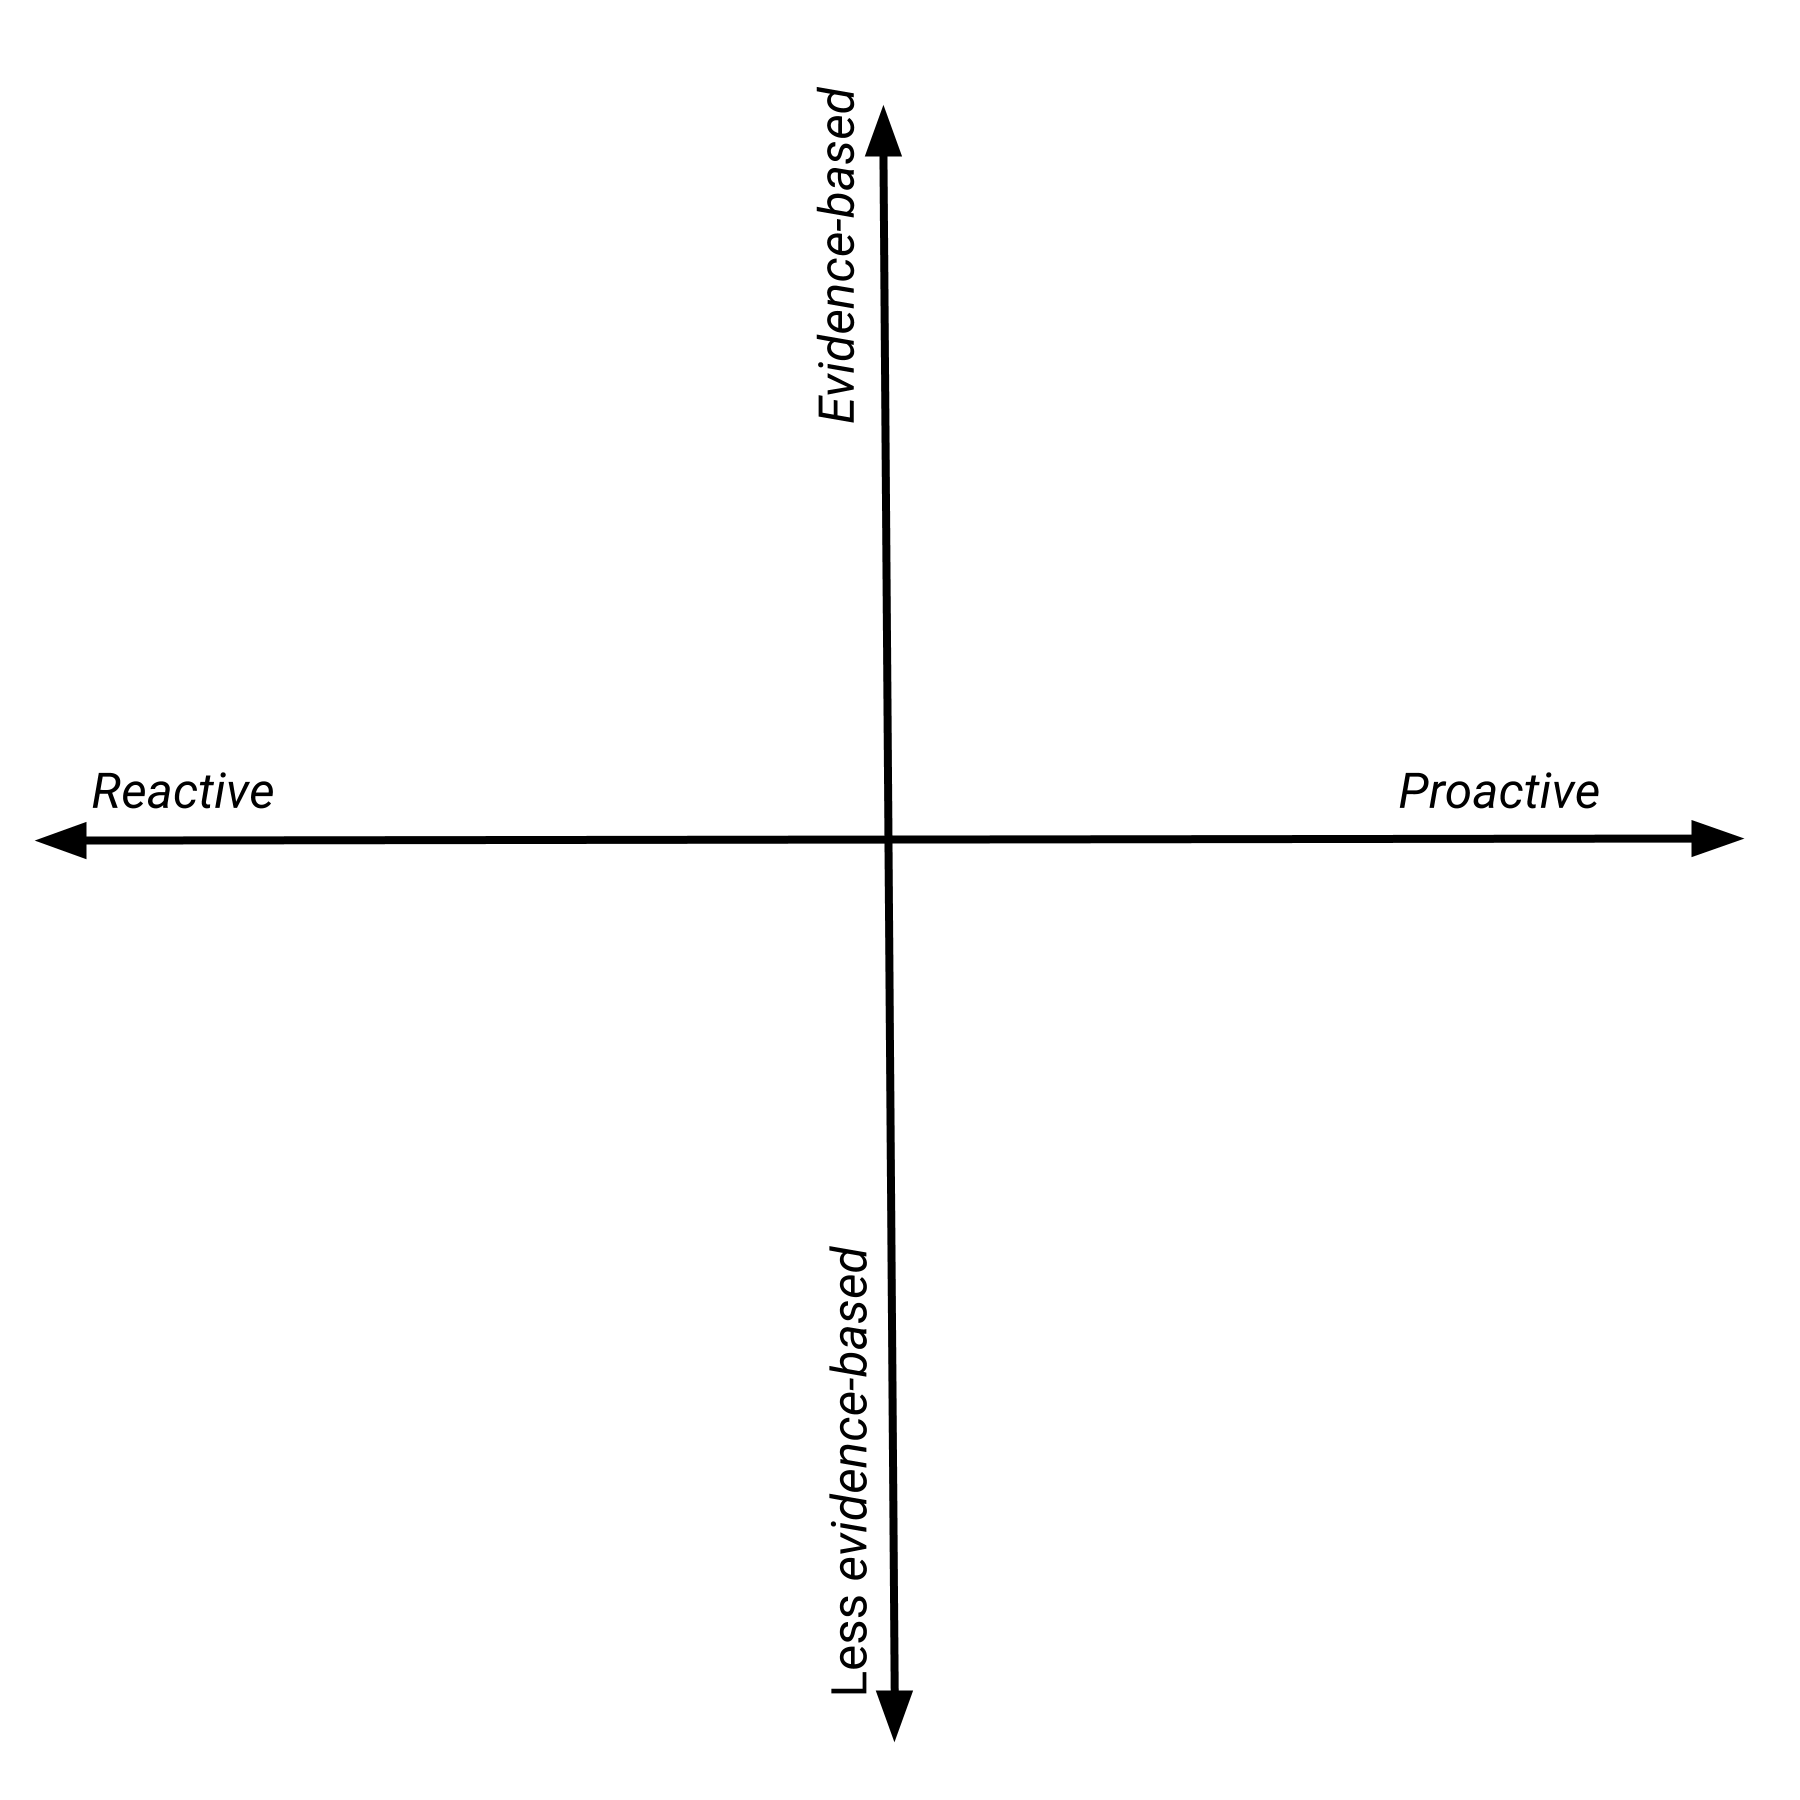
\includegraphics{files/CMEthics_context3.png}
\caption{Participants tended to vary according to how they approached
complementary medicines and how they approached evidence
\label{context3}}
\end{figure}

\subsubsection{Navigating practice in a retail
environment}\label{navigating-practice-in-a-retail-environment}

All participants discussed implications of the retail environment within
the context of fulfilling their professional obligations. Participants
who were pharmacy owners, in particular, recognised the impact of
complementary medicines on the financial bottom-line of the pharmacy.

\begin{quote}
I own a pharmacy \ldots{} I still work in the shop on a daily basis. So
I still come across on a daily basis having to chat to people about
this. But them I am also going to come at it from the side {[}that
complementary medicines{]} prop up half of the bank loan. So I guess we
are going to go both ways on this a little bit. (D5P7)
\end{quote}

Participants differed, however, in how they navigated practice in the
retail environment. Most participants sought to prioritize professional
obligations over financial considerations.

\begin{quote}
If a pharmacy's going to lose money for the sake of a sale, that isn't a
good enough reason for the sake of giving something out. We should
always be having a look at evidence-based treatments, \ldots{} (D4P5)
\end{quote}

These participants focused on ensuring appropriate practice within the
confines of financial constraints. Because participants differed in how
they viewed appropriate practice in the context of complementary
medicines, they also differed on the financial impost they were willing
to accept to fulfil the responsibilities outlined in the proposed
framework. This topic is discussed in detail below in relation to the
acceptability and feasibility of the framework.

\subsection{Context}\label{context}

Participants described how they approached complementary medicines in
day-to-day interactions with consumers as well as how they thought
pharmacists \emph{should} approach such interactions. They also
discussed what resources they had available to them to assist consumers
with complementary medicines as well as any barriers they experienced
when providing advice to consumers in relation to complementary
medicines. Topics frequently raised by participants in focus groups and
interviews were the role of naturopaths in community pharmacy, the
availability of resources on complementary medicines and the increasing
role of practitioner-only complementary medicine lines. How participants
approached these topics was informed by the approach they took to
complementary medicines and their views regarding evidence. These views
are summarised in Figure~\ref{fig_context2}.

\begin{figure}
\centering
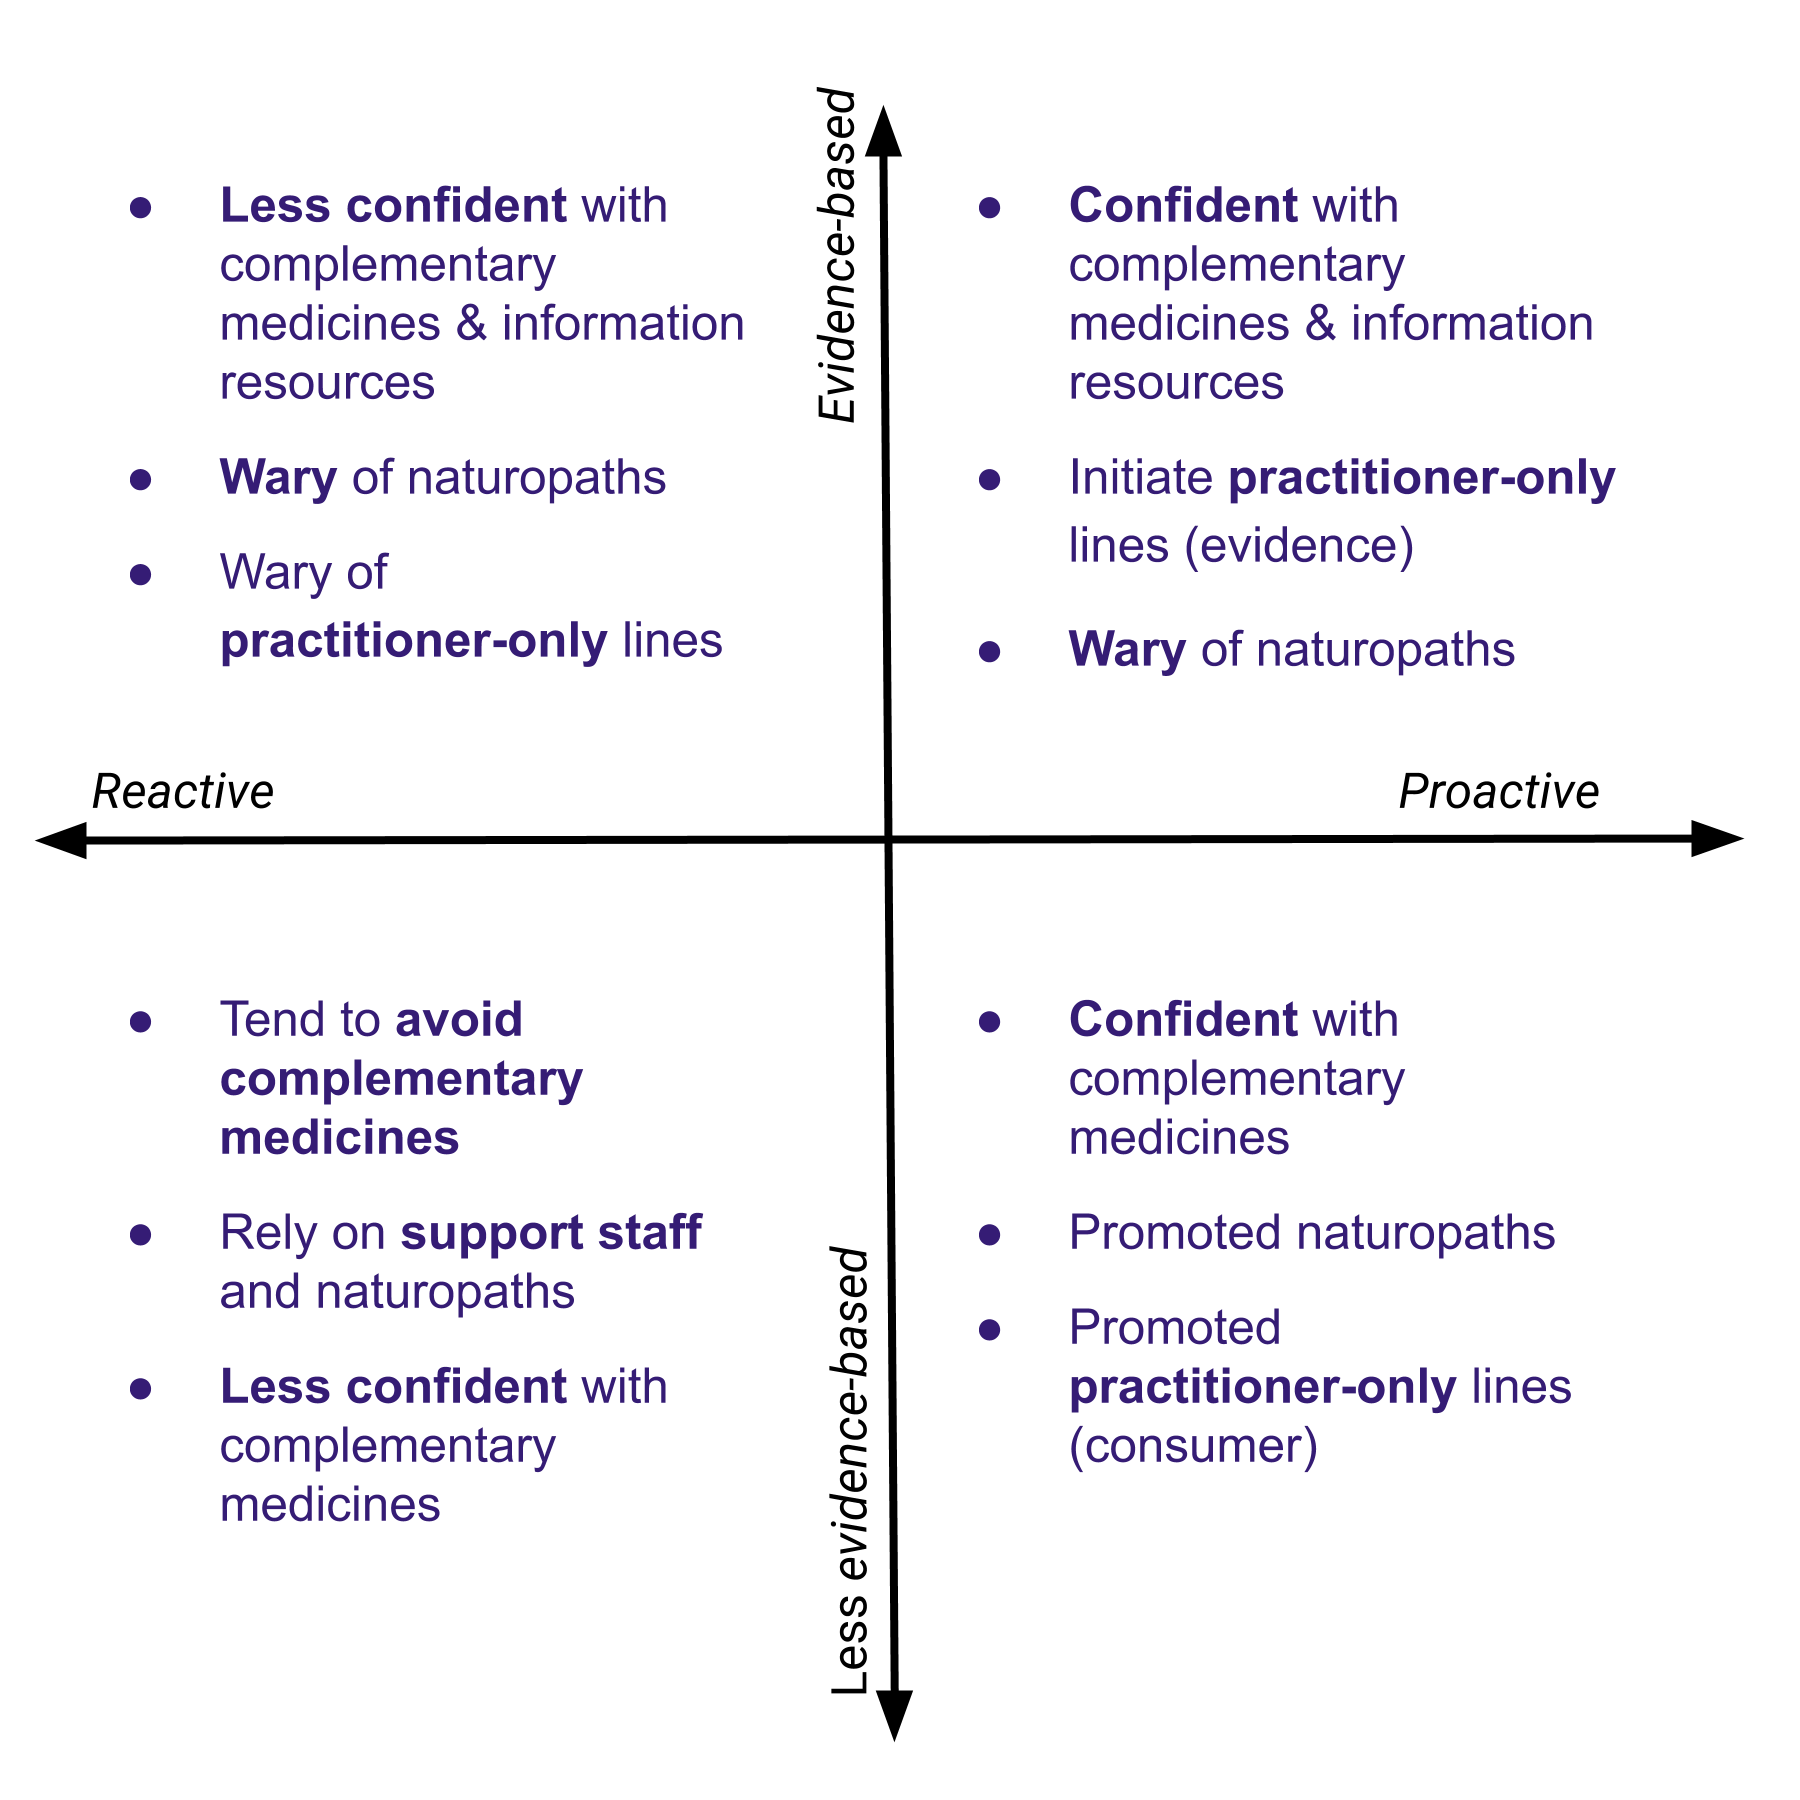
\includegraphics{files/CMEthics_context2.png}
\caption{How participants varied in relation to how they viewed the
context of providing advice on complementary medicines in community
pharmacy \label{fig_context2}}
\end{figure}

\subsubsection{Naturopaths in community
pharmacy}\label{naturopaths-in-community-pharmacy}

Participants expressed a range of attitudes in relation to the role of
naturopaths in community pharmacy. Participants with a greater focus on
evidence-based practice tended see the benefits in having a naturopath
in-store that shared that focus. However, only some of these
participants found that the naturopaths they worked with had an
evidence-based focus.

\begin{quote}
My take on it is, surely pharmacists and naturopaths should,
essentially, have the same information, the same evidence. We should
come to the same conclusions. Now there's going to be better and perhaps
not so great professionals in both industries. There's going to be
differing opinions, but that's just healthy science. Surely we should
cooperate. There's definitely room for both, and there's definitely room
for businesses that see the value of a great naturopath\ldots{}. (D5P9)

\ldots{}{[}I{]}s that the experience you've had, that naturopaths are
coming from the same perspective? (AL)

Personally, the one that I had, absolutely not\ldots{}. The guy, if he
didn't know he would just make it up. And I do not run that sort of
pharmacy, so that immediately rubbed me the wrong way. (D5P9)
\end{quote}

A common source of contention for participants with a focus on
evidence-based practice, was the tendency of naturopaths to recommend
homeopathy.

\begin{quote}
In terms of naturopaths, I have no faith in homoeopathic products from
everything that I've learned at university, which was quite a long time
ago. Yeah. I don't trust homoeopathic products. So I would never
recommend a homoeopathic product, and I would question the use of a
homoeopathic product. So in terms of that and naturopaths in pharmacy, I
would be quite uncomfortable with that. (D9P15)
\end{quote}

Participants who talked about practice in ways that were less
evidence-based, such as those who relied on placebo effects or put
considerable weight on anecdotal reports, tended to be more supportive
of the role of naturopaths in community pharmacy. These participants
were inclined to view the knowledge of naturopaths as complementary to
the knowledge pharmacists, with both professionals sharing a similar
overall perspective with differing areas of expertise. Some of these
participants also noted the benefits that having a good naturopath in
the pharmacy can have on sales.

\begin{quote}
The naturopaths have done the studies of all the herbs and everything
else where the pharmacists just get a basic top knowledge. So I think
that the naturopaths know a lot more because they've been taught and
they've had to do research. Whether we're getting the same, I don't
think pharmacists have the in-depth knowledge to go deeply into all the
herbs and everything else, all the complementary medicines. So some
would, but at this point in time, I don't see any training out there for
pharmacists to help their knowledge in depth. So I would say the
naturopath has a lot more than the pharmacists. But working together -
we have the drug knowledge; they have the complementary knowledge -
helping people to live a better life combined would be awesome. (D8P14)
\end{quote}

\begin{quote}
\ldots{}
\end{quote}

\begin{quote}
We used to have a naturopath but they're really hard to get and keep. I
know that one of our other stores has a naturopath and we will, quite
often, ring and ask them for advice. I think that they have a lot more
knowledge in this area. And if you can get one into store, it can boost
your sales considerably and boost the confidence that people have in
that area because they do have that knowledge. And then backing them up
if they have questions with medications and things like that, the
pharmacist can back them up. But I think that if you can get a
naturopath you can develop your complementary medicine area really quite
nicely. (D8P14)
\end{quote}

\subsubsection{Information resources on complementary
medicines}\label{information-resources-on-complementary-medicines}

Participants views on the information resources available in community
pharmacy differed according to their approach to complementary medicines
and approach to evidence. Participants with a proactive approach to
complementary medicines and who had an evidence-based focus in their
practice frequently had a range of information resources available to
them (some of them paid for by the pharmacy), which they were confident
in using and they found helpful.

\begin{quote}
Also, I think a really important resource I use is on the Natural
Standard database. So especially when looking at interactions like if
someone's on blood pressure medication, you can easily see whether or
not they should be-- yeah. If there's interactions and it also gives you
level of evidence as well, like mild, moderate, that sort of thing.
(D7P13)
\end{quote}

Other resources included access to information provided by particular
manufacturers, especially manufacturers of practitioner-only lines.

\begin{quote}
I guess, we all use Dr.~Google. Probably not for the best. I guess, some
companies are better. I know BioCeuticals, we have one of their massive
books which, if we need to look something up, gives us a really good
guideline. Some of the companies-- I think Nature's Own has a hotline.
Blackmores may have a hotline that you can actually ring and ask and
speak to somebody. But it's all time-consuming. And in this day and age,
a lot of people don't want that time-consuming job. (D8P14)
\end{quote}

Participants who took a more reactive approach to complementary
medicines were more likely to express a desire for more access to better
resources.

\begin{quote}
I feel like it would be really helpful if there was a better database to
look up interactions and all that type of thing because more often than
not, I have to call either the company or look into it really far to
make sure it doesn't interact. (D3P4)
\end{quote}

\subsubsection{Practitioner-only lines}\label{practitioner-only-lines}

Practitioner-only lines have typically been sold by naturopaths working
in the pharmacy, but in recent years pharmacists have become more
actively involved in these sales. Most of these complementary medicines
are regulated in the same way as complementary medicines sold in the
front shop, but are marketed such that only certain practitioners can
sell the item (typically naturopaths and pharmacists). Several
participants described a high level of activity in personally selling
and recommending practitioner-only lines. See, for example, the second
quote in Section~\ref{approach-to-complementary-medicines}. Most of
these participants had an evidence-based focus in their practice and
were proactive in relation to complementary medicines. These
participants saw practitioner-only lines as a way to support and provide
evidence-based complementary medicines, with many of the companies
selling these product providing resources to support their sale.

\begin{quote}
I think we also sort of need to look at the practitioner-only ones and
those companies out there that are doing good research and seeing what
sort of role they play as well because I think, at the moment, they are
a good thing that is available, but a lot of consumers don't know about
it, and they might buy a cheaper fish oil from the supermarket.
Obviously, they could still buy the cheaper product, but I mean, I think
there's something to look into there as well. (D2P3)
\end{quote}

\subsection{Acceptability and feasibility of the
framework}\label{acceptability-and-feasibility-of-the-framework}

Most participants felt the framework was acceptable: that it accurately
captured the responsibilities of pharmacists when selling complementary
medicines. Participants were more likely to express concern regarding
the feasibility of the framework. Participant views on the acceptability
and feasibility of the framework tended to be informed by how they
approached complementary medicines and how they approached evidence. The
other key determinant was how the participant navigated practice within
a retail environment.

The main perceived threat to the acceptability of the framework that was
expressed by a small number of participants was the cost impost to
pharmacists of implementing the framework when other retailers of
complementary medicines are not obligated to provide the same services.
This view was most strongly expressed by participants who were reactive
in relation to complementary medicines and tended to be less
evidence-based. Within focus groups this view was directly challenged by
other participants who felt that it was appropriate for pharmacies to
compete on services and cost as opposed to cost alone. Participant views
regarding the acceptability and feasibility of the framework are
summarised in Figure~\ref{accfeas}.

\begin{figure}
\centering
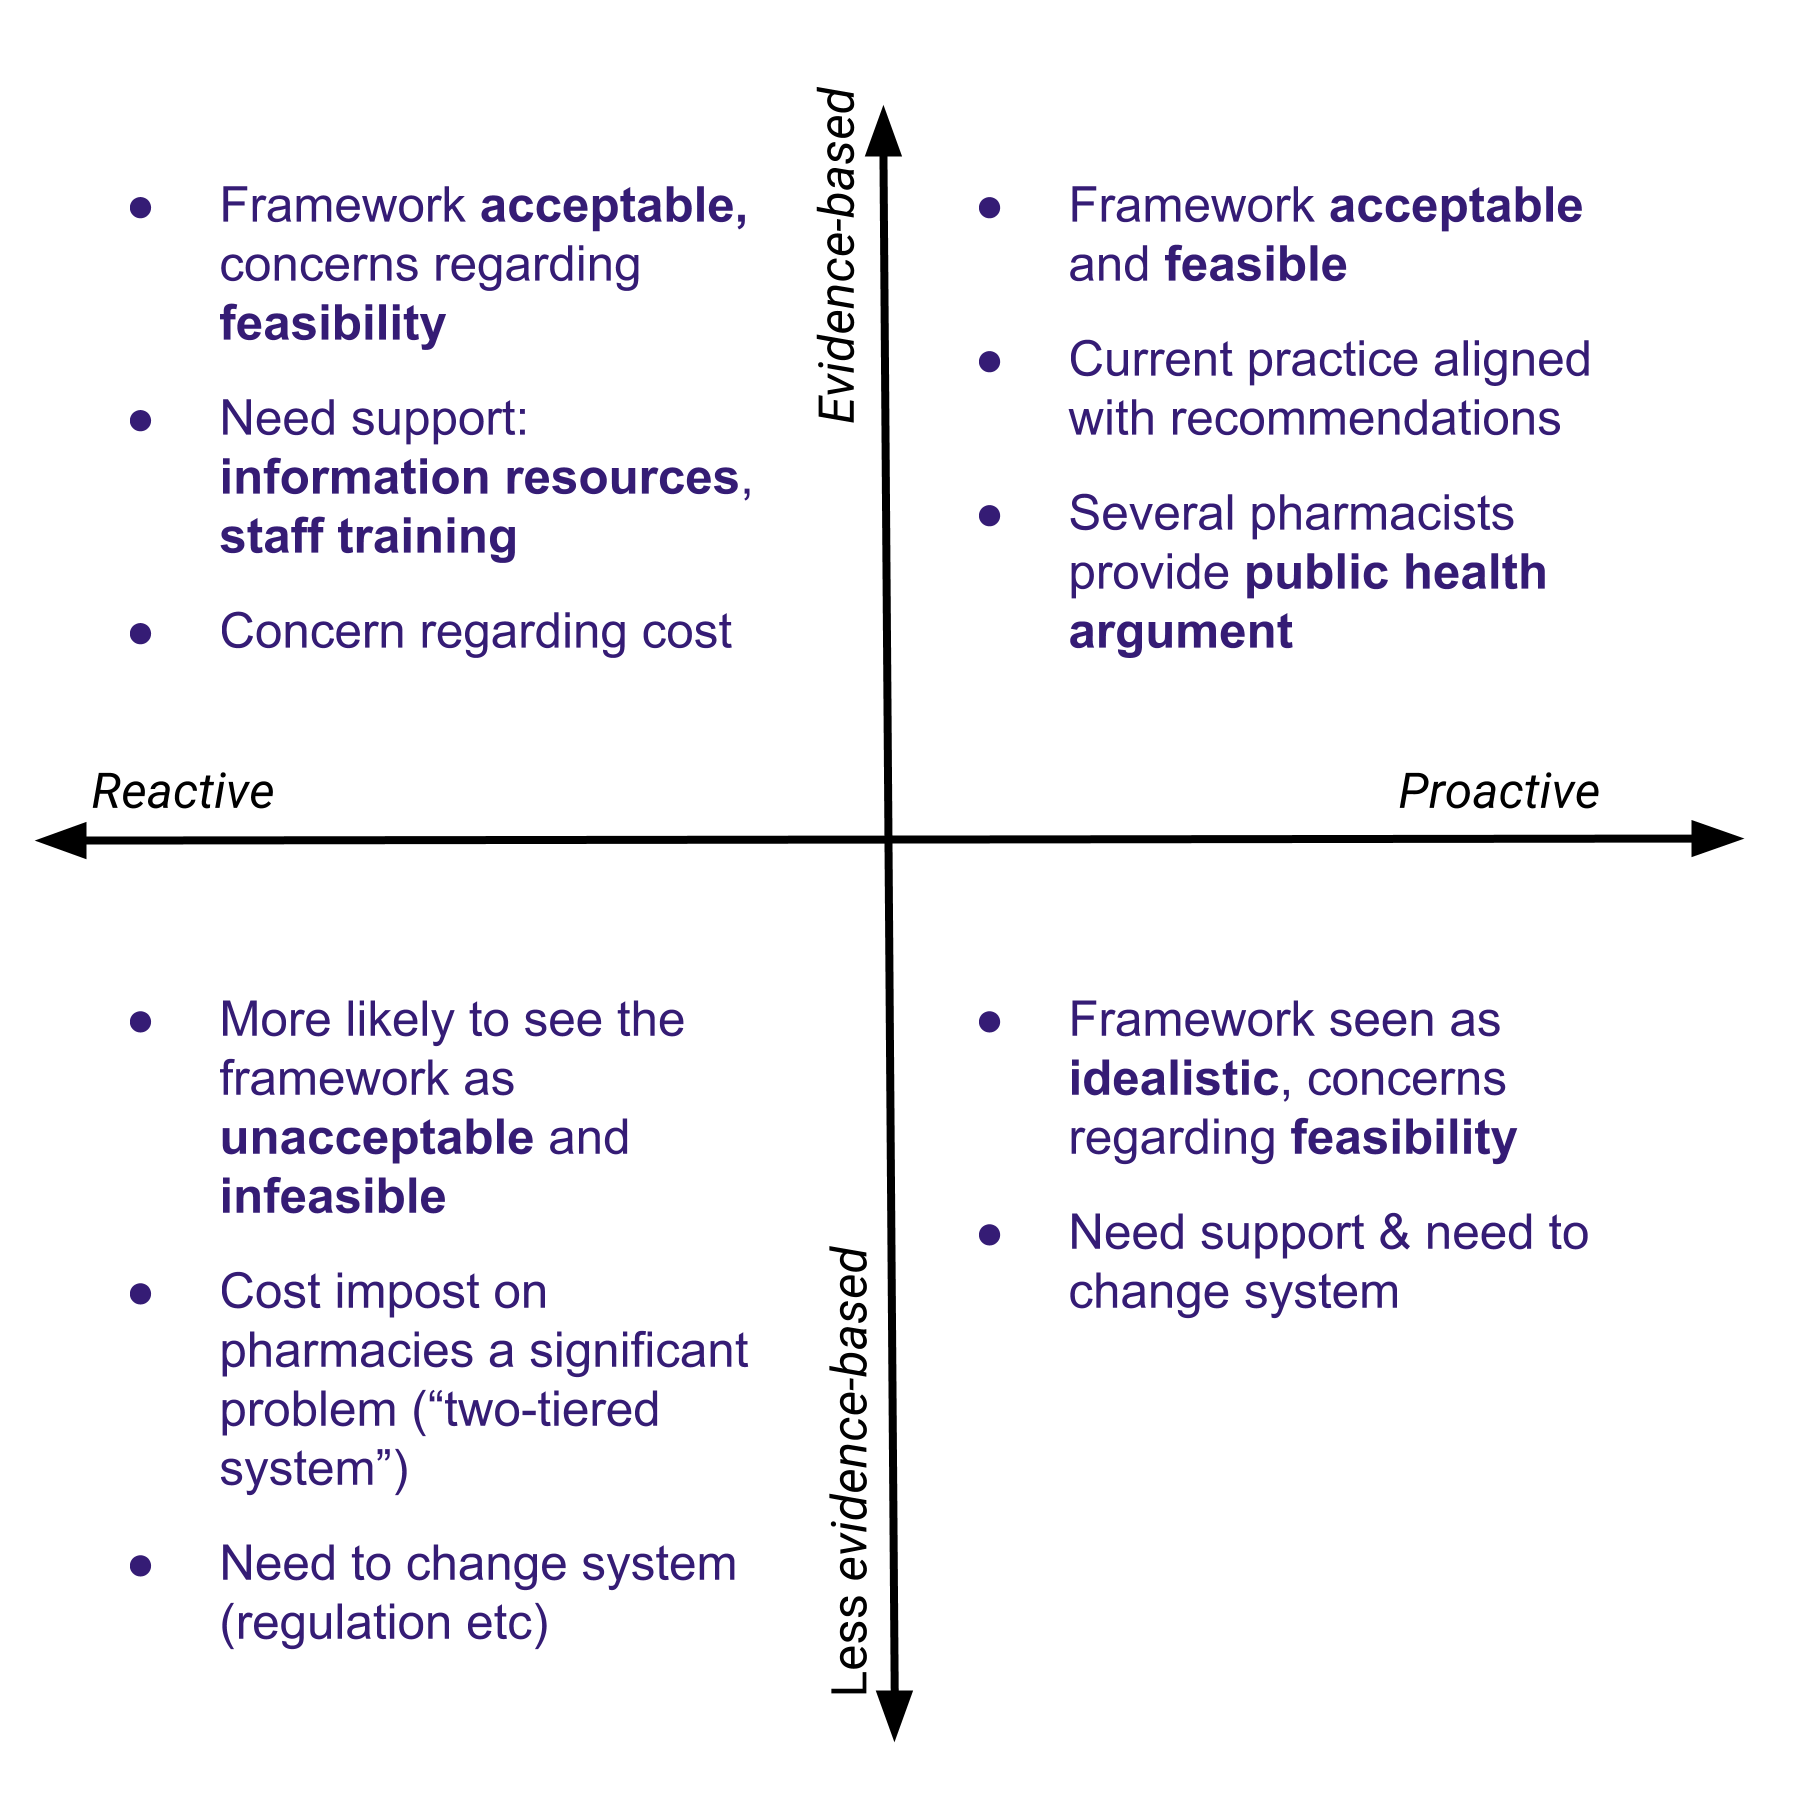
\includegraphics{files/CMEthics_accfeas.png}
\caption{How participants views on the acceptability and feasibility of
the framework different depending on how they approach complementary
medicines and evidence \label{accfeas}}
\end{figure}

\subsubsection{Acceptability}\label{acceptability}

The majority of participants felt the framework was acceptable,
especially those who were ``proactive'' \emph{or} ``evidence-based''.
Participants who were ``proactive'' and ``evidence-based'' were most
strongly in favour of the proposed ethical framework. These participants
saw the framework as a being closely aligned with their practice and
commended the clear guidance the framework provided regarding pharmacist
responsibilities when selling complementary medicines.

\begin{quote}
I think generally pharmacists are time poor and stressed and
overburdened, so anything that can make something more simplified and
streamlined with clear-cut expectations is useful. (D7P12)
\end{quote}

\begin{quote}
\ldots{}
\end{quote}

\begin{quote}
I would say {[}the framework is acceptable{]}, particularly with, yeah,
treating it along the lines of an S2 or an S3. So front-shop staff can
talk to the patients about it. If there's any further queries, the
pharmacist can be involved, but they don't automatically have to come
down and talk to them if it's not something that there's any questions
about. (D7P11)
\end{quote}

Several participants provided an argument along the lines of the public
health argument to support the sale of complementary medicines in
community pharmacies.

\begin{quote}
I think the reason that pharmacies should sell their complementary
medicine is not because there is a market. I think people, instead of
going to the health food store to get their {[}comple?{]} medicine, they
should come to the pharmacy because there is a better chance that the
pharmacies can find out if there's any interaction for people with some
actual medications. But I know most of my customers. I know exactly what
they are taking. If they come and someone on warfarin asks me for some
complementary medication, I just quickly before going and checking their
medical history, I know that that's not the right thing to give to the
person. But if that person goes to the health food store and buy it
there, there is no way that they can figure it out. So I think they
should be always at the pharmacy because people should think to go to
pharmacy to get their complementary medicine because that way they are
going to be protected and lots of trauma is going to be stopped. (D1P1)
\end{quote}

Two threats to acceptability were identified in the focus groups and
interviews. The primary perceived threat to the acceptability of the
framework was that it permits a ``two-tiered system'' for the sale of
complementary medicines. The framework identifies responsibilities for
pharmacies selling complementary medicines that are not expected of
other retailers. This point was raised in several focus groups and
interviews. The following quotes illustrate the back-and-forth between a
participant who argues the framework is not acceptable due to the
differential cost it imposes on community pharmacies and a second
participant who argues that part of being a pharmacist involves such
obligations.

\begin{quote}
I would say consumers mostly view {[}complementary medicines{]} as an
item of commerce. You buy them like you buy bread and milk, in some
instances, for some of them. So you've now imposed this cost on us
providing evidence, but in order to do that, we have to mark the product
up more. Then you've got this two-tiered system. (D5P7)
\end{quote}

\begin{quote}
I think that having the degree means that \ldots{} people come for a
higher level of service and understanding than what they can get in the
supermarket. And that's part of what differentiates us professionally.
And that's part of why it's still called a pharmacy and not a
supermarket. I'm comfortable that I would actually be probably more
comfortable practising where the TGA just says, ``Yes, that is safe to
take.'' And then the pharmacist makes the clinical judgement and says,
``Well, this may not be the best product for you.'' I think that that's
literally our goal. (D5P9)
\end{quote}

The second threat to the acceptability of the framework is a consequence
of the different approaches participants take to evidence-based practice
in relation to complementary medicines. The proposed framework assumes a
shared understanding of what is considered appropriate evidence for the
efficacy of complementary medicines. The framework adopts an approach to
medical evidence that recognises both the importance of well designed
trials in providing evidence that taking a complementary medicine
produces the expected benefits and a sound scientific understanding of
the mechanisms by which the complementary medicine by benefit or cause
harm \autocite{Parkkinen2018a}.

This threat was not explicitly raised by participants but the importance
of recognising it can be

\subsubsection{Feasibility}\label{feasibility}

\printbibliography[title=References]

\end{document}
